\documentclass[12pt,a4paper]{scrartcl}\usepackage[]{graphicx}\usepackage[]{color}
%% maxwidth is the original width if it is less than linewidth
%% otherwise use linewidth (to make sure the graphics do not exceed the margin)
\makeatletter
\def\maxwidth{ %
  \ifdim\Gin@nat@width>\linewidth
    \linewidth
  \else
    \Gin@nat@width
  \fi
}
\makeatother

\definecolor{fgcolor}{rgb}{0.345, 0.345, 0.345}
\newcommand{\hlnum}[1]{\textcolor[rgb]{0.686,0.059,0.569}{#1}}%
\newcommand{\hlstr}[1]{\textcolor[rgb]{0.192,0.494,0.8}{#1}}%
\newcommand{\hlcom}[1]{\textcolor[rgb]{0.678,0.584,0.686}{\textit{#1}}}%
\newcommand{\hlopt}[1]{\textcolor[rgb]{0,0,0}{#1}}%
\newcommand{\hlstd}[1]{\textcolor[rgb]{0.345,0.345,0.345}{#1}}%
\newcommand{\hlkwa}[1]{\textcolor[rgb]{0.161,0.373,0.58}{\textbf{#1}}}%
\newcommand{\hlkwb}[1]{\textcolor[rgb]{0.69,0.353,0.396}{#1}}%
\newcommand{\hlkwc}[1]{\textcolor[rgb]{0.333,0.667,0.333}{#1}}%
\newcommand{\hlkwd}[1]{\textcolor[rgb]{0.737,0.353,0.396}{\textbf{#1}}}%
\let\hlipl\hlkwb

\usepackage{framed}
\makeatletter
\newenvironment{kframe}{%
 \def\at@end@of@kframe{}%
 \ifinner\ifhmode%
  \def\at@end@of@kframe{\end{minipage}}%
  \begin{minipage}{\columnwidth}%
 \fi\fi%
 \def\FrameCommand##1{\hskip\@totalleftmargin \hskip-\fboxsep
 \colorbox{shadecolor}{##1}\hskip-\fboxsep
     % There is no \\@totalrightmargin, so:
     \hskip-\linewidth \hskip-\@totalleftmargin \hskip\columnwidth}%
 \MakeFramed {\advance\hsize-\width
   \@totalleftmargin\z@ \linewidth\hsize
   \@setminipage}}%
 {\par\unskip\endMakeFramed%
 \at@end@of@kframe}
\makeatother

\definecolor{shadecolor}{rgb}{.97, .97, .97}
\definecolor{messagecolor}{rgb}{0, 0, 0}
\definecolor{warningcolor}{rgb}{1, 0, 1}
\definecolor{errorcolor}{rgb}{1, 0, 0}
\newenvironment{knitrout}{}{} % an empty environment to be redefined in TeX

\usepackage{alltt}
\usepackage[utf8]{inputenc}
\usepackage{amsmath}
\usepackage{graphicx}
\usepackage{tikz}
%\usepackage{silence}
\usepackage{mdframed}
%\WarningFilter{mdframed}{You got a bad break}
\usepackage[colorinlistoftodos]{todonotes}
\usepackage{listings}
\usepackage{color}
\colorlet{exampcol}{blue!10}
\usepackage{multicol}
\usepackage{booktabs}

\usepackage[]{exercise}%[noanswer]

\usepackage[autostyle, english = american]{csquotes}
\MakeOuterQuote{"}

\usepackage{hyperref}
\hypersetup{
    colorlinks,
    citecolor=black,
    filecolor=black,
    linkcolor=blue,
    urlcolor=blue
}

\title{Exercises for ``Multiple regression"}
\date{\today}
\author{Timoth\'ee Bonnet}
%\institute{BDSI / RSB}
\IfFileExists{upquote.sty}{\usepackage{upquote}}{}
\begin{document}



\maketitle

Find the content for today and previous workshops at \href{https://github.com/timotheenivalis/RSB-R-Stats-Biology}{https://github.com/timotheenivalis/RSB-R-Stats-Biology}.

\tableofcontents
\ListOfExerciseInToc
\ExerciseLevelInToc{subsubsection}

\clearpage 

\section{Multiple regression}

\begin{Exercise}[difficulty=1, title={Jumping}]
  \begin{enumerate}
    \item load \texttt{jumpingdistance.csv}. It contains jumping distances by people of different masses and heights. 
    \item Use plots and lm() to test whether mass increases or decreases jumping distance. Based on the classical mechanics what do you expect?
  \end{enumerate}


\end{Exercise}
\begin{Answer}
\begin{knitrout}
\definecolor{shadecolor}{rgb}{0.969, 0.969, 0.969}\color{fgcolor}\begin{kframe}
\begin{alltt}
  \hlstd{jumping} \hlkwb{<-} \hlkwd{read.csv}\hlstd{(}\hlkwc{file} \hlstd{=} \hlstr{"jumpingdistance.csv"}\hlstd{)}
\end{alltt}
\end{kframe}
\end{knitrout}

A first approach suggests mass increases jumping distance:
\begin{knitrout}
\definecolor{shadecolor}{rgb}{0.969, 0.969, 0.969}\color{fgcolor}\begin{kframe}
\begin{alltt}
    \hlkwd{summary}\hlstd{(}\hlkwd{lm}\hlstd{(jump} \hlopt{~} \hlstd{mass,} \hlkwc{data}\hlstd{=jumping))}
    \hlkwd{plot}\hlstd{(mass, jump)}
\end{alltt}
\end{kframe}
\end{knitrout}

But that is incorrect and due to the correlation between mass and height:
\begin{knitrout}
\definecolor{shadecolor}{rgb}{0.969, 0.969, 0.969}\color{fgcolor}\begin{kframe}
\begin{alltt}
    \hlkwd{summary}\hlstd{(}\hlkwd{lm}\hlstd{(jump} \hlopt{~} \hlstd{mass} \hlopt{+} \hlstd{height,} \hlkwc{data}\hlstd{=jumping))}
\end{alltt}
\end{kframe}
\end{knitrout}
The direct (causal) effect of mass is negative, as revealed by a multiple regression.

The NET effect of mass is positive, but conditional on height mass as a negative effect.
\end{Answer}

\begin{Exercise}[difficulty=1, title={Babies}]



    \begin{enumerate}
      \item Load \texttt{babies.csv}
      \item What drives change in number of babies born?
    \end{enumerate}
\end{Exercise}
\begin{Answer}
\begin{knitrout}
\definecolor{shadecolor}{rgb}{0.969, 0.969, 0.969}\color{fgcolor}\begin{kframe}
\begin{alltt}
  \hlstd{babies} \hlkwb{<-} \hlkwd{read.csv}\hlstd{(}\hlstr{"babies.csv"}\hlstd{)}
  \hlkwd{summary}\hlstd{(}\hlkwd{lm}\hlstd{(babies_born} \hlopt{~} \hlstd{number_of_storks,} \hlkwc{data} \hlstd{= babies))}
\end{alltt}
\begin{verbatim}
## 
## Call:
## lm(formula = babies_born ~ number_of_storks, data = babies)
## 
## Residuals:
##    Min     1Q Median     3Q    Max 
## -1.723 -0.634 -0.286  0.572  2.302 
## 
## Coefficients:
##                  Estimate Std. Error t value Pr(>|t|)    
## (Intercept)       14.4569     0.1747   82.74   <2e-16 ***
## number_of_storks   0.0886     0.0161    5.51    1e-06 ***
## ---
## Signif. codes:  0 '***' 0.001 '**' 0.01 '*' 0.05 '.' 0.1 ' ' 1
## 
## Residual standard error: 1.03 on 54 degrees of freedom
## Multiple R-squared:  0.36,	Adjusted R-squared:  0.348 
## F-statistic: 30.4 on 1 and 54 DF,  p-value: 1.02e-06
\end{verbatim}
\begin{alltt}
  \hlkwd{summary}\hlstd{(}\hlkwd{lm}\hlstd{(babies_born} \hlopt{~} \hlstd{number_of_storks} \hlopt{+} \hlstd{year,} \hlkwc{data} \hlstd{= babies))}
\end{alltt}
\begin{verbatim}
## 
## Call:
## lm(formula = babies_born ~ number_of_storks + year, data = babies)
## 
## Residuals:
##    Min     1Q Median     3Q    Max 
## -1.871 -0.686 -0.178  0.769  2.124 
## 
## Coefficients:
##                  Estimate Std. Error t value Pr(>|t|)   
## (Intercept)      -72.3262    27.9141   -2.59    0.012 * 
## number_of_storks   0.0196     0.0268    0.73    0.468   
## year               0.0439     0.0141    3.11    0.003 **
## ---
## Signif. codes:  0 '***' 0.001 '**' 0.01 '*' 0.05 '.' 0.1 ' ' 1
## 
## Residual standard error: 0.953 on 53 degrees of freedom
## Multiple R-squared:  0.459,	Adjusted R-squared:  0.438 
## F-statistic: 22.5 on 2 and 53 DF,  p-value: 8.64e-08
\end{verbatim}
\begin{alltt}
  \hlkwd{summary}\hlstd{(}\hlkwd{lm}\hlstd{(babies_born} \hlopt{~} \hlstd{year,} \hlkwc{data} \hlstd{= babies))}
\end{alltt}
\begin{verbatim}
## 
## Call:
## lm(formula = babies_born ~ year, data = babies)
## 
## Residuals:
##    Min     1Q Median     3Q    Max 
## -1.922 -0.675 -0.208  0.723  2.133 
## 
## Coefficients:
##              Estimate Std. Error t value Pr(>|t|)    
## (Intercept) -89.21206   15.58519   -5.72  4.7e-07 ***
## year          0.05246    0.00784    6.69  1.3e-08 ***
## ---
## Signif. codes:  0 '***' 0.001 '**' 0.01 '*' 0.05 '.' 0.1 ' ' 1
## 
## Residual standard error: 0.948 on 54 degrees of freedom
## Multiple R-squared:  0.453,	Adjusted R-squared:  0.443 
## F-statistic: 44.8 on 1 and 54 DF,  p-value: 1.31e-08
\end{verbatim}
\begin{alltt}
  \hlkwd{summary}\hlstd{(}\hlkwd{lm}\hlstd{(babies_born} \hlopt{~} \hlstd{mean_temperature}\hlopt{+} \hlstd{year,} \hlkwc{data} \hlstd{= babies))}
\end{alltt}
\begin{verbatim}
## 
## Call:
## lm(formula = babies_born ~ mean_temperature + year, data = babies)
## 
## Residuals:
##    Min     1Q Median     3Q    Max 
## -1.941 -0.665 -0.194  0.711  2.106 
## 
## Coefficients:
##                  Estimate Std. Error t value Pr(>|t|)    
## (Intercept)      -86.4347    17.3717   -4.98  7.2e-06 ***
## mean_temperature   0.2482     0.6626    0.37     0.71    
## year               0.0494     0.0113    4.38  5.7e-05 ***
## ---
## Signif. codes:  0 '***' 0.001 '**' 0.01 '*' 0.05 '.' 0.1 ' ' 1
## 
## Residual standard error: 0.956 on 53 degrees of freedom
## Multiple R-squared:  0.455,	Adjusted R-squared:  0.434 
## F-statistic: 22.1 on 2 and 53 DF,  p-value: 1.05e-07
\end{verbatim}
\begin{alltt}
  \hlkwd{summary}\hlstd{(}\hlkwd{lm}\hlstd{(babies_born} \hlopt{~} \hlstd{mean_temperature}\hlopt{+} \hlstd{number_of_storks} \hlopt{+} \hlstd{year,} \hlkwc{data} \hlstd{= babies))}
\end{alltt}
\begin{verbatim}
## 
## Call:
## lm(formula = babies_born ~ mean_temperature + number_of_storks + 
##     year, data = babies)
## 
## Residuals:
##    Min     1Q Median     3Q    Max 
## -1.889 -0.656 -0.185  0.721  2.101 
## 
## Coefficients:
##                  Estimate Std. Error t value Pr(>|t|)  
## (Intercept)      -70.5229    28.7193   -2.46    0.017 *
## mean_temperature   0.2124     0.6678    0.32    0.752  
## number_of_storks   0.0189     0.0271    0.70    0.488  
## year               0.0416     0.0160    2.61    0.012 *
## ---
## Signif. codes:  0 '***' 0.001 '**' 0.01 '*' 0.05 '.' 0.1 ' ' 1
## 
## Residual standard error: 0.961 on 52 degrees of freedom
## Multiple R-squared:  0.46,	Adjusted R-squared:  0.429 
## F-statistic: 14.7 on 3 and 52 DF,  p-value: 4.51e-07
\end{verbatim}
\end{kframe}
\end{knitrout}
\end{Answer}


\begin{Exercise}[difficulty=2, title={Bird abundance}]
Loyn (1987) modeled the abundance of forest birds with six predictor variables (patch area, distance to nearest patch, distance to nearest larger patch, grazing intensity, altitude and years since the patch had been isolated).
That is a classical example wrongly analyses in textbooks (they tend to say that the initial analysis was wrong because of correlations between predictors\dots however linear models do not make assumptions about correlations among predictors, as long as the correlations are not 1 or -1).
Load the dataset \texttt{loyn.csv}. Think of a reasonable causal model that would predict bird abundance. 
Before rushing to fit models, look at the distributions of variables, some of them may benefit from a log-transformation (for practical convenience and for logic both!).
Test it using an appropriate multiple regression. Also try a model containing all predictors. Compare your results to that of a series of simple regressions (one for each of your predictors). Try to understand the differences.
\end{Exercise}
\begin{Answer}  
\begin{knitrout}
\definecolor{shadecolor}{rgb}{0.969, 0.969, 0.969}\color{fgcolor}\begin{kframe}
\begin{alltt}
\hlstd{birds} \hlkwb{<-} \hlkwd{read.csv}\hlstd{(}\hlstr{"loyn.csv"}\hlstd{)}
\hlkwd{plot}\hlstd{(birds)}
\end{alltt}
\end{kframe}
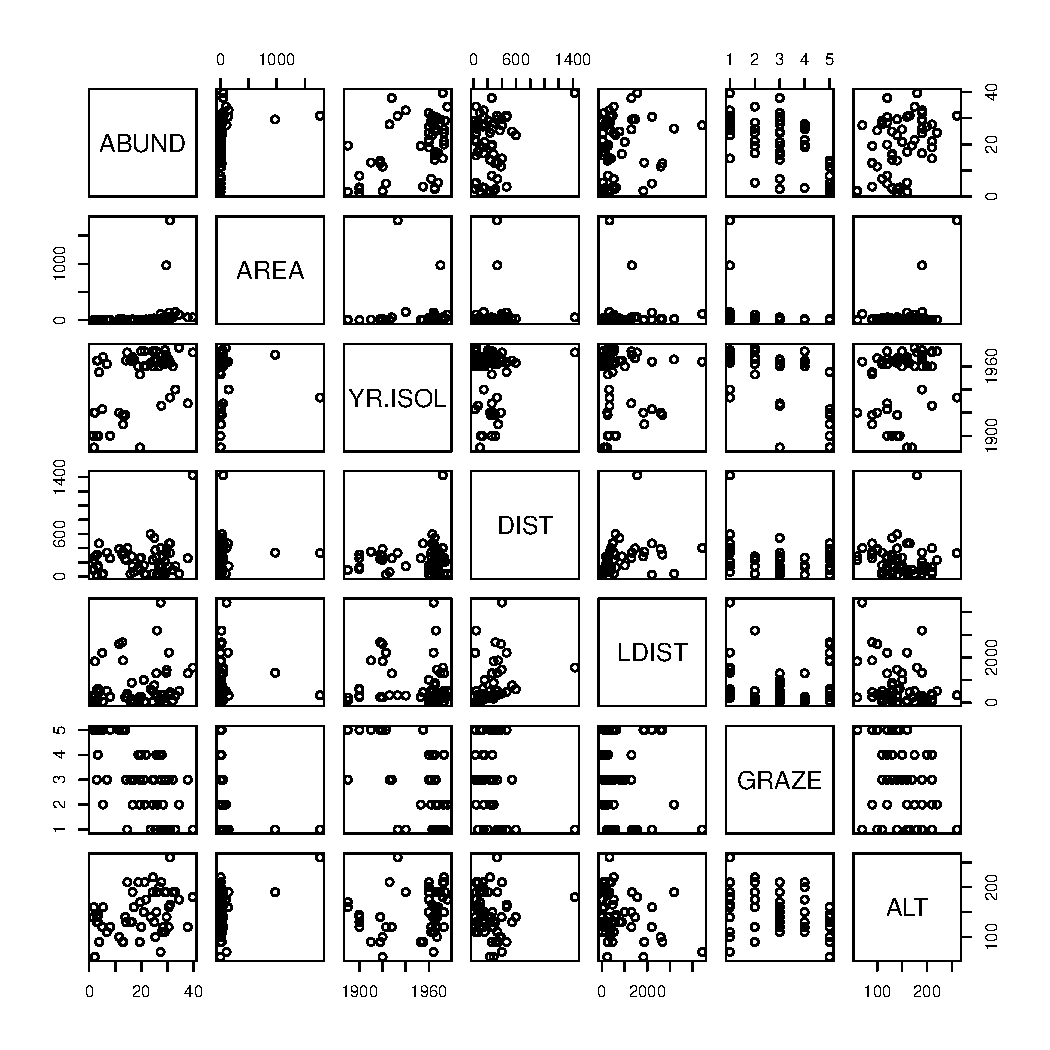
\includegraphics[width=\maxwidth]{figure/unnamed-chunk-9-1} 
\begin{kframe}\begin{alltt}
\hlkwd{summary}\hlstd{(}\hlkwd{lm}\hlstd{(ABUND} \hlopt{~} \hlnum{1} \hlopt{+} \hlkwd{log}\hlstd{(AREA)} \hlopt{+} \hlstd{YR.ISOL} \hlopt{+} \hlstd{ALT} \hlopt{+} \hlkwd{log}\hlstd{(LDIST)} \hlopt{+} \hlkwd{as.factor}\hlstd{(GRAZE),} \hlkwc{data} \hlstd{= birds))}
\end{alltt}
\begin{verbatim}
## 
## Call:
## lm(formula = ABUND ~ 1 + log(AREA) + YR.ISOL + ALT + log(LDIST) + 
##     as.factor(GRAZE), data = birds)
## 
## Residuals:
##    Min     1Q Median     3Q    Max 
## -15.80  -2.78  -0.37   2.78  11.21 
## 
## Coefficients:
##                   Estimate Std. Error t value Pr(>|t|)    
## (Intercept)        36.7039   113.9498    0.32   0.7488    
## log(AREA)           2.9642     0.6454    4.59  3.3e-05 ***
## YR.ISOL            -0.0125     0.0574   -0.22   0.8286    
## ALT                 0.0103     0.0234    0.44   0.6618    
## log(LDIST)          0.3972     0.8195    0.48   0.6302    
## as.factor(GRAZE)2   0.3897     3.0117    0.13   0.8976    
## as.factor(GRAZE)3  -0.0494     2.7716   -0.02   0.9859    
## as.factor(GRAZE)4  -1.3218     3.1080   -0.43   0.6726    
## as.factor(GRAZE)5 -12.5640     4.6693   -2.69   0.0098 ** 
## ---
## Signif. codes:  0 '***' 0.001 '**' 0.01 '*' 0.05 '.' 0.1 ' ' 1
## 
## Residual standard error: 6.04 on 47 degrees of freedom
## Multiple R-squared:  0.729,	Adjusted R-squared:  0.683 
## F-statistic: 15.8 on 8 and 47 DF,  p-value: 5.12e-11
\end{verbatim}
\end{kframe}
\end{knitrout}
Suggests area as a strong and clear effect. Very strong grazing does have a negative effect. There is no clear statistical support for altitude and year of isolation.

Simple regressions of these two predictors show significant effects though:
\begin{knitrout}
\definecolor{shadecolor}{rgb}{0.969, 0.969, 0.969}\color{fgcolor}\begin{kframe}
\begin{alltt}
\hlkwd{summary}\hlstd{(}\hlkwd{lm}\hlstd{(ABUND} \hlopt{~} \hlnum{1} \hlopt{+} \hlstd{YR.ISOL ,} \hlkwc{data} \hlstd{= birds))}
\end{alltt}
\begin{verbatim}
## 
## Call:
## lm(formula = ABUND ~ 1 + YR.ISOL, data = birds)
## 
## Residuals:
##     Min      1Q  Median      3Q     Max 
## -19.835  -6.113   0.506   5.831  22.780 
## 
## Coefficients:
##              Estimate Std. Error t value Pr(>|t|)    
## (Intercept) -392.3208    96.2143   -4.08  0.00015 ***
## YR.ISOL        0.2112     0.0493    4.28  7.7e-05 ***
## ---
## Signif. codes:  0 '***' 0.001 '**' 0.01 '*' 0.05 '.' 0.1 ' ' 1
## 
## Residual standard error: 9.36 on 54 degrees of freedom
## Multiple R-squared:  0.253,	Adjusted R-squared:  0.24 
## F-statistic: 18.3 on 1 and 54 DF,  p-value: 7.68e-05
\end{verbatim}
\begin{alltt}
\hlkwd{summary}\hlstd{(}\hlkwd{lm}\hlstd{(ABUND} \hlopt{~} \hlnum{1} \hlopt{+} \hlstd{ALT,} \hlkwc{data} \hlstd{= birds))}
\end{alltt}
\begin{verbatim}
## 
## Call:
## lm(formula = ABUND ~ 1 + ALT, data = birds)
## 
## Residuals:
##     Min      1Q  Median      3Q     Max 
## -19.023  -7.562   0.006   8.573  20.683 
## 
## Coefficients:
##             Estimate Std. Error t value Pr(>|t|)   
## (Intercept)   5.5983     4.7209    1.19   0.2409   
## ALT           0.0952     0.0310    3.07   0.0033 **
## ---
## Signif. codes:  0 '***' 0.001 '**' 0.01 '*' 0.05 '.' 0.1 ' ' 1
## 
## Residual standard error: 9.99 on 54 degrees of freedom
## Multiple R-squared:  0.149,	Adjusted R-squared:  0.133 
## F-statistic: 9.45 on 1 and 54 DF,  p-value: 0.00332
\end{verbatim}
\end{kframe}
\end{knitrout}

That's probably due to their correlation with grazing pressure:
\begin{knitrout}
\definecolor{shadecolor}{rgb}{0.969, 0.969, 0.969}\color{fgcolor}\begin{kframe}
\begin{alltt}
\hlkwd{summary}\hlstd{(}\hlkwd{lm}\hlstd{(YR.ISOL} \hlopt{~} \hlnum{1} \hlopt{+} \hlkwd{as.factor}\hlstd{(GRAZE) ,} \hlkwc{data} \hlstd{= birds))}
\end{alltt}
\begin{verbatim}
## 
## Call:
## lm(formula = YR.ISOL ~ 1 + as.factor(GRAZE), data = birds)
## 
## Residuals:
##    Min     1Q Median     3Q    Max 
## -63.67  -4.86   4.50   8.33  41.62 
## 
## Coefficients:
##                   Estimate Std. Error t value Pr(>|t|)    
## (Intercept)        1962.62       4.31  454.99  < 2e-16 ***
## as.factor(GRAZE)2     4.76       6.99    0.68     0.50    
## as.factor(GRAZE)3    -8.95       5.89   -1.52     0.14    
## as.factor(GRAZE)4     2.24       7.29    0.31     0.76    
## as.factor(GRAZE)5   -49.23       6.10   -8.07  1.1e-10 ***
## ---
## Signif. codes:  0 '***' 0.001 '**' 0.01 '*' 0.05 '.' 0.1 ' ' 1
## 
## Residual standard error: 15.6 on 51 degrees of freedom
## Multiple R-squared:  0.657,	Adjusted R-squared:  0.63 
## F-statistic: 24.4 on 4 and 51 DF,  p-value: 2.46e-11
\end{verbatim}
\begin{alltt}
\hlkwd{summary}\hlstd{(}\hlkwd{lm}\hlstd{(ALT} \hlopt{~} \hlnum{1} \hlopt{+} \hlkwd{as.factor}\hlstd{(GRAZE),} \hlkwc{data} \hlstd{= birds))}
\end{alltt}
\begin{verbatim}
## 
## Call:
## lm(formula = ALT ~ 1 + as.factor(GRAZE), data = birds)
## 
## Residuals:
##    Min     1Q Median     3Q    Max 
## -91.92 -22.94   0.58  28.08  98.08 
## 
## Coefficients:
##                   Estimate Std. Error t value Pr(>|t|)    
## (Intercept)         161.92      10.98   14.74   <2e-16 ***
## as.factor(GRAZE)2     7.45      17.80    0.42   0.6772    
## as.factor(GRAZE)3   -15.92      15.01   -1.06   0.2937    
## as.factor(GRAZE)4    -5.49      18.57   -0.30   0.7685    
## as.factor(GRAZE)5   -50.77      15.53   -3.27   0.0019 ** 
## ---
## Signif. codes:  0 '***' 0.001 '**' 0.01 '*' 0.05 '.' 0.1 ' ' 1
## 
## Residual standard error: 39.6 on 51 degrees of freedom
## Multiple R-squared:  0.232,	Adjusted R-squared:  0.172 
## F-statistic: 3.86 on 4 and 51 DF,  p-value: 0.00818
\end{verbatim}
\end{kframe}
\end{knitrout}
so they correlate with abundance, but the correlation is likely driven by a direct effect of grazing.

\end{Answer}
\end{document}
